\section{Создание программного средства}
\label{sec:creation}

Исходя из опыта работы разработчика и поставленной задачи целесообразное всего использовать язык \csharp{} платформы \dotnet{}.

В разделе \ref{sec:arch_arch} была рассмотренна архитектура програмного средства и было определенно что разные части приложения буду иметь следующую архитекуру:
\begin{itemize}
	\item клиен-сервер
	\item каналы и фильтры
	\item микроядерная архитектура
\end{itemize}
Рассмотрим технические средства помогающие реализовать приведенный функционал.

Для реализации програмного средства как клиент-сервер можно использовать следующие фреймворки:
\begin{itemize}
	\item ASP.NET MVC
	\item NancyFx
\end{itemize}
Оба фреймовка предоставляют отличный возможности для создания веб приложений, но я выбрал именно nancyFx из-за его простого развертывания. Для запуска NancyFx можно использовать IIS, WCF и OWIN.

Для реализации каналов и фильтров пока нету готовых фреймворков, есть лишь пример реализации архитектурного шаблона от Microsoft для платформы c использованием языка \csharp{} \cite{pipes_and_filters_pattern}, на рисунке \ref{fig:creation:pipes_and_filters_microsoft} можно увидеть схему работы шаблона.

\begin{figure}[ht] 
    \centering
    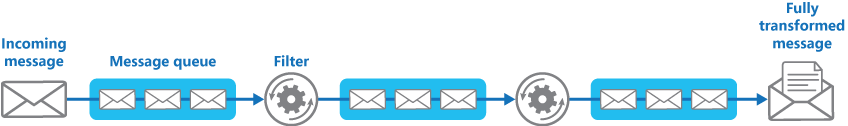
\includegraphics[scale=0.5]{pipes_and_filters_microsoft.png}  
    \caption{Схема реализации шаблона <<Каналы и фильтры>> от Microsoft}
    \label{fig:creation:pipes_and_filters_microsoft}
\end{figure}

Описанная реализация фокусируется на возможности распределенных вычислений которая в контексте обработки изображений бесполезно, поскольку производительность полученная от распределения фильтров на различные машины будет нивелированна временем затраченным передачу обрабатываемого изображения по сети. Главная цель использования шаблона <<Каналы и фильтры>> это улучшение качества кода с точки зрения читаемости и модифицируемости. Декомпозиция кода на отдельные фильтры обработчики помогает упростить тестирование и реализацию отдельных модулей а правильная реализация каналов поможет в понимании связи фильтров и того что в целом происходит при обработке изображения. 

\begin{lstlisting}[style=csharpstyle, caption={Пример автоматического вывода типа функции}, label=lst:creation:pipes_example]
Mat binarizedPlate = null;
return _processFactory.Invoke()
	.Use(input)
    .Do<ReadImageFromBytesProcessor, Mat>()
    .Do<MakeImageGrayProcessor, Mat>()
    .Do<DetectAndCropPlateNumberProcessor, IEnumerable<Mat>>()
    .ForEachItem(p => 
        p.Do<LogCurrentImageProcessor, Mat>()
        .Do<OtsuBinarizationProcessor, Mat>()
        .SaveCurrentResultTo(r => binarizedPlate = r.Value.Clone())
        .Do<InvertBinarizedImageProcessor, Mat>()
        .Do<FindContoursProcessor, Point[][]>()
        .Do<SelectLettersContours, Point[][]>(processor => processor.UseImage(binarizedPlate))
        .Do<CropLettersProcessor, IEnumerable<Mat>>(processor => processor.UseImage(binarizedPlate))
        .ForEachItem(ip => ip.Do<GaussianBlurProcessor, Mat>().Do<TeseractOcrProcessor, char>()))
        .Do<StringAgregateProcessor, IEnumerable<string>>()
        .GetResult();
\end{lstlisting}